\documentclass[a4paper]{article}
\usepackage[a4paper, margin=1in]{geometry}
% Some basic packages
\usepackage[utf8]{inputenc}
\usepackage[T1]{fontenc}
\usepackage{textcomp}
\usepackage[dutch]{babel}
\usepackage{url}
\usepackage{graphicx}
\usepackage{float}
\usepackage{booktabs}
\usepackage{enumitem}

\pdfminorversion=7

% Don't indent paragraphs, leave some space between them
\usepackage{parskip}

% Hide page number when page is empty
\usepackage{emptypage}
\usepackage{subcaption}
\usepackage{multicol}
\usepackage{xcolor}

% Other font I sometimes use.
% \usepackage{cmbright}

% Math stuff
\usepackage{amsmath, amsfonts, mathtools, amsthm, amssymb}
% Fancy script capitals
\usepackage{mathrsfs}
\usepackage{cancel}
% Bold math
\usepackage{bm}
% Some shortcuts
\newcommand\N{\ensuremath{\mathbb{N}}}
\newcommand\R{\ensuremath{\mathbb{R}}}
\newcommand\Z{\ensuremath{\mathbb{Z}}}
\renewcommand\O{\ensuremath{\emptyset}}
\newcommand\Q{\ensuremath{\mathbb{Q}}}
\newcommand\C{\ensuremath{\mathbb{C}}}

% Easily typeset systems of equations (French package)
\usepackage{systeme}

% Put x \to \infty below \lim
\let\svlim\lim\def\lim{\svlim\limits}

%Make implies and impliedby shorter
\let\implies\Rightarrow
\let\impliedby\Leftarrow
\let\iff\Leftrightarrow
\let\epsilon\varepsilon

% Add \contra symbol to denote contradiction
\usepackage{stmaryrd} % for \lightning
\newcommand\contra{\scalebox{1.5}{$\lightning$}}

% \let\phi\varphi

% Command for short corrections
% Usage: 1+1=\correct{3}{2}

\definecolor{correct}{HTML}{009900}
\newcommand\correct[2]{\ensuremath{\:}{\color{red}{#1}}\ensuremath{\to }{\color{correct}{#2}}\ensuremath{\:}}
\newcommand\green[1]{{\color{correct}{#1}}}

% horizontal rule
\newcommand\hr{
    \noindent\rule[0.5ex]{\linewidth}{0.5pt}
}

% hide parts
\newcommand\hide[1]{}

% si unitx
\usepackage{siunitx}
\sisetup{locale = FR}

% Environments
\makeatother
% For box around Definition, Theorem, \ldots
\usepackage{mdframed}
\mdfsetup{skipabove=1em,skipbelow=0em}
\theoremstyle{definition}
\newmdtheoremenv[nobreak=true]{definitie}{Definitie}
\newmdtheoremenv[nobreak=true]{eigenschap}{Eigenschap}
\newmdtheoremenv[nobreak=true]{gevolg}{Gevolg}
\newmdtheoremenv[nobreak=true]{lemma}{Lemma}
\newmdtheoremenv[nobreak=true]{propositie}{Propositie}
\newmdtheoremenv[nobreak=true]{stelling}{Stelling}
\newmdtheoremenv[nobreak=true]{wet}{Wet}
\newmdtheoremenv[nobreak=true]{postulaat}{Postulaat}
\newmdtheoremenv{conclusie}{Conclusie}
\newmdtheoremenv{toemaatje}{Toemaatje}
\newmdtheoremenv{vermoeden}{Vermoeden}
\newtheorem*{herhaling}{Herhaling}
\newtheorem*{intermezzo}{Intermezzo}
\newtheorem*{notatie}{Notatie}
\newtheorem*{observatie}{Observatie}
\newtheorem*{oef}{Oefening}
\newtheorem*{opmerking}{Opmerking}
\newtheorem*{praktisch}{Praktisch}
\newtheorem*{probleem}{Probleem}
\newtheorem*{terminologie}{Terminologie}
\newtheorem*{toepassing}{Toepassing}
\newtheorem*{uovt}{UOVT}
\newtheorem*{vb}{Voorbeeld}
\newtheorem*{vraag}{Vraag}

\newmdtheoremenv[nobreak=true]{definition}{Definition}
\newtheorem*{eg}{Example}
\newtheorem*{notation}{Notation}
\newtheorem*{previouslyseen}{As previously seen}
\newtheorem*{remark}{Remark}
\newtheorem*{note}{Note}
\newtheorem*{problem}{Problem}
\newtheorem*{observe}{Observe}
\newtheorem*{property}{Property}
\newtheorem*{intuition}{Intuition}
\newmdtheoremenv[nobreak=true]{prop}{Proposition}
\newmdtheoremenv[nobreak=true]{theorem}{Theorem}
\newmdtheoremenv[nobreak=true]{corollary}{Corollary}

% End example and intermezzo environments with a small diamond (just like proof
% environments end with a small square)
\usepackage{etoolbox}
\AtEndEnvironment{vb}{\null\hfill$\diamond$}%
\AtEndEnvironment{intermezzo}{\null\hfill$\diamond$}%
% \AtEndEnvironment{opmerking}{\null\hfill$\diamond$}%

% Fix some spacing
% http://tex.stackexchange.com/questions/22119/how-can-i-change-the-spacing-before-theorems-with-amsthm
\makeatletter
\def\thm@space@setup{%
  \thm@preskip=\parskip \thm@postskip=0pt
}


% Exercise 
% Usage:
% \oefening{5}
% \suboefening{1}
% \suboefening{2}
% \suboefening{3}
% gives
% Oefening 5
%   Oefening 5.1
%   Oefening 5.2
%   Oefening 5.3
\newcommand{\oefening}[1]{%
    \def\@oefening{#1}%
    \subsection*{Oefening #1}
}

\newcommand{\suboefening}[1]{%
    \subsubsection*{Oefening \@oefening.#1}
}


% \lecture starts a new lecture (les in dutch)
%
% Usage:
% \lecture{1}{di 12 feb 2019 16:00}{Inleiding}
%
% This adds a section heading with the number / title of the lecture and a
% margin paragraph with the date.

% I use \dateparts here to hide the year (2019). This way, I can easily parse
% the date of each lecture unambiguously while still having a human-friendly
% short format printed to the pdf.

\usepackage{xifthen}
\def\testdateparts#1{\dateparts#1\relax}
\def\dateparts#1 #2 #3 #4 #5\relax{
    \marginpar{\small\textsf{\mbox{#1 #2 #3 #5}}}
}

\def\@lecture{}%
\newcommand{\lecture}[3]{
    \ifthenelse{\isempty{#3}}{%
        \def\@lecture{Lecture #1}%
    }{%
        \def\@lecture{Lecture #1: #3}%
    }%
    \subsection*{\@lecture}
    \marginpar{\small\textsf{\mbox{#2}}}
}



% These are the fancy headers
\usepackage{fancyhdr}
\pagestyle{fancy}

% LE: left even
% RO: right odd
% CE, CO: center even, center odd
% My name for when I print my lecture notes to use for an open book exam.
% \fancyhead[LE,RO]{Gilles Castel}

\fancyhead[RO,LE]{\@lecture} % Right odd,  Left even
\fancyhead[RE,LO]{}          % Right even, Left odd

\fancyfoot[RO,LE]{\thepage}  % Right odd,  Left even
\fancyfoot[RE,LO]{}          % Right even, Left odd
\fancyfoot[C]{\leftmark}     % Center

\makeatother




% Todonotes and inline notes in fancy boxes
\usepackage{todonotes}
\usepackage{tcolorbox}

% Make boxes breakable
\tcbuselibrary{breakable}

% Verbetering is correction in Dutch
% Usage: 
% \begin{verbetering}
%     Lorem ipsum dolor sit amet, consetetur sadipscing elitr, sed diam nonumy eirmod
%     tempor invidunt ut labore et dolore magna aliquyam erat, sed diam voluptua. At
%     vero eos et accusam et justo duo dolores et ea rebum. Stet clita kasd gubergren,
%     no sea takimata sanctus est Lorem ipsum dolor sit amet.
% \end{verbetering}
\newenvironment{verbetering}{\begin{tcolorbox}[
    arc=0mm,
    colback=white,
    colframe=green!60!black,
    title=Opmerking,
    fonttitle=\sffamily,
    breakable
]}{\end{tcolorbox}}

% Noot is note in Dutch. Same as 'verbetering' but color of box is different
\newenvironment{noot}[1]{\begin{tcolorbox}[
    arc=0mm,
    colback=white,
    colframe=white!60!black,
    title=#1,
    fonttitle=\sffamily,
    breakable
]}{\end{tcolorbox}}




% Figure support as explained in my blog post.
\usepackage{import}
\usepackage{xifthen}
\usepackage{pdfpages}
\usepackage{transparent}
\newcommand{\incfig}[1]{%
    \def\svgwidth{\columnwidth}
    \import{./figures/}{#1.pdf_tex}
}

% Fix some stuff
% %http://tex.stackexchange.com/questions/76273/multiple-pdfs-with-page-group-included-in-a-single-page-warning
\pdfsuppresswarningpagegroup=1

\title{\Huge{Hw 7}}
\author{\huge{Daniel Yu}}
\date{October 27, 2024}

\pdfsuppresswarningpagegroup=1

\begin{document}
\maketitle
\newpage% or \cleardoublepage
% \pdfbookmark[<level>]{<title>}{<dest>}
\pagebreak

\begin{enumerate}
  \item You enter a casino with 100 dollars, and continuously play a fair game: each minute, you either
gain a dollar with probability 1/2, or lose a dollar with probability 1/2. You leave the casino when
you are out of money, or after you have 400 dollars. What is the probability that you leave the
casino with no money.

\begin{proof}
  We will denote $q_i = P[\text{leave the casino with no money } \mid \text{intial wealth is $i$}]$. Then,
  \begin{itemize}
    \item $q_0 = 1$
    \item $q_1 = \frac{1}{2} q_0 + \frac{1}{2} q_2$ (probability you lose your only dollar + probability you lose all from 2 dollars)
    \item $q_2 = \frac{1}{2} q_1 + \frac{1}{2} q_3$ (probability you lose to go to $q_1$ + probability you win to go to go to 3 dollars and lose all)
    \item $q_3 = \frac{1}{2} q_2 + \frac{1}{2} q_4$ 
    \item $\ldots$
    \item $q_{400}= 0$
  \end{itemize}
  We want to solve for $q_{100}$.  
  \begin{align*}
    q_{100} &= \frac{1}{2} q_{99} + \frac{1}{2} q_{101} \\
            &= \frac{1}{2} \left( \frac{1}{2}q_{98} + \frac{1}{2} q_{100} \right)  + \frac{1}{2} \left( \frac{1}{2} q_{100} + \frac{1}{2} q_{102} \right) \\
            &= \frac{1}{2} \left(\frac{1}{2} (\frac{1}{2} q_{97} + \frac{1}{2} q_{99}) + \frac{1}{2} (\frac{1}{2}q_{99} + \frac{1}{2} q_{101})\right) + \frac{1}{2} \left( \frac{1}{2} (\frac{1}{2}q_{99} + \frac{1}{2} q_{101}) + \frac{1}{2} ( \frac{1}{2} q_{101}  + \frac{1}{2} q_{103} ) \right)  \\
            &= \ldots
  .\end{align*}
  Notice the linear relationship: 
  $$q_{100} = \frac{1}{2}^{k} \sum_{i=1}^{2^{k - 1}} q_{100 -k + 2i} + \frac{1}{2}^{k} \sum_{i=1}^{2^{k-1}} q_{100 + k - 2i}$$. This gets extremely complicated. \\

  We know that that the probability is symmetric for a random walk starting from $q_{200}$, i.e. $q_{200} = \frac{1}{2}$. Since $q_i$ is a random walk,  and only depends on $q_{i+1}$,  we can see that the probability would continue to be symmetric. Notice that $$q_{i} = \frac{1}{2}q_{i-1} + \frac{1}{2} q_{i+1} \Rightarrow 2q_i = q_{i-1} + q_{i+1} \Rightarrow q_i - q_{i-1} = q_{i+1} - q_i$$. 
  This implies that the probability is an arthimetic series and thus the relationship between terms is linear as there is some constant $q_i = q_{i-1} + c, \forall i \in 1,\ldots,400$! Thus, $q_i = q_{0} + c \cdot i = 1 + c \cdot i$. Substitute, $i=400$
  \[
  q_{400} = 0 = 1 - c \cdot 400 \Rightarrow c = \frac{1}{400}
  .\] 
  and,
  \[
  q_i = 1 - \frac{i}{400}
  .\] 

Thus, $q_{100} =$ the number of steps from the $q_{400}$ over the total steps = $\frac{300}{400} = \frac{3}{4}$

\end{proof}
\item Let a, b be two numbers between 0 and 1. Consider the two-state Markov chain given by the
transition probabilities
\[
 P_{a,b}= \begin{pmatrix} 1 -a &  a \\ b & 1 - b \end{pmatrix}
.\] 
\begin{enumerate}
  \item For what values of a and b is this chain irreducible?
\begin{proof}
  Transition matrices $P$ are irreducible when $a=1$ and  $b=1$ or when  $0 < a < 1$ and  $0 < b < 1$. When $a=1, b=1$ $P = \begin{pmatrix} 0 &  1 \\ 1 & 0 \end{pmatrix}$, then $P^{2} = I$ identity matrix, so $P$ is still irreducible since it is possible to get from any state to any other state in 2 steps. However, when  $P = I$ and $a=0,b=0$, then there is no way to travel from 1 state or the other, so  $P$ is not irreducible. Finally, when $0 < a < 1, 0 < b<1$, then it is possible to get to any state to any other state in 1 step, so  $P$ is irreducible.
\end{proof}
  \item For what values of a and b is it aperiodic?
\begin{proof}
  The transition matrix $P$ changes slightly for the markov chain to be aperiodic. $P$ when $a=1, b=1$ is no longer a valid transition matrix for a aperiodic markov chain, in fact in this case there is a period of $2$. The matrix  $P$ are of the forms  $0 < a <1, 0 < b < 1$ since $P^{N}$ with $N = 1$ now satisfies the periodicity condition and clearly the matrix is also aperiodic when  $a =0, b=0$ as the period is 1.
\end{proof}

  \item Assuming a and b satisfy the conditions required for the chain to be irreducible, find the stationary distribution of the Markov chain (as a function of a and b)
\begin{proof}
  We would find the eigenvector associated with one. 
  \begin{align*}
    \vec{v} \cdot P_{a,b} &= 1 \cdot \vec{v} \\
    \vec{v}  \begin{pmatrix} 1 -a &  a \\ b & 1 - b \end{pmatrix} &=  \vec{v} \\
    \begin{pmatrix} x & y \end{pmatrix}  \begin{pmatrix} 1 -a &  a \\ b & 1 - b \end{pmatrix} &=  \begin{pmatrix} x & y \end{pmatrix}  \\
    \begin{pmatrix} (1-a) x + b y & ax + (1-b) y \end{pmatrix}  &= \begin{pmatrix} x & y \end{pmatrix}   
  .\end{align*}
  We know that:
  \begin{align*}
    (1-a)x + by &= x \\
    ax + (1-b)y &= y \\
    x + y &= 1
  .\end{align*}
  Solving,
  \begin{align}
    x &= 1 - y \\
    -ax + by &= 0 \\
    -a(1-y) + by &= 0 \\
    -a +ay + by &= 0 \\
    y(a+b) &= a \\
    y &= \frac{a}{a+b} \\
    x &= \frac{b}{a+b}
  .\end{align}
  Thus,
  \[
    \vec{v}^{T} = \begin{pmatrix} \frac{b}{a+b} \\ \frac{a}{a+b} \end{pmatrix} 
  .\] 
\end{proof}
\end{enumerate}
  
\item We say a matrix is doubly stochastic if both the rows and columns of the matrix sum up to one.
Let P be a doubly stochastic matrix that is the transition probability matrix for a Markov chain
with N states. Find a stationary distribution for this Markov chain.

\begin{proof}
  Let $P$ be the doubly stochastic matrix that is the transition probability matrix for the markov chain with  $N$ states. This means that the rows and columns of  $P$ both sum to 1 and all entries are non-negative. From class we proved that $Null(P-I) = span \{\vec{1}\}$ i.e. $P \cdot \vec{1} = \vec{1}$. We can then consider $P^{T}$ which must now be row-stochastic, so by the same theorem  $Null(P^{T}-I) = \span {\vec{1}}$ and  $P^{T} \cdot \vec{1} = \vec{1}$. By transpose law,
  \[
    P^{T} \cdot \vec{1} \Rightarrow \vec{1}^{T} P = \vec{1}^{T} 
  .\] 
  Thus, the constant vector is a row-eigenvector and thus a stationary distribution for this markov chain.
\end{proof}

\item Construct a Markov chain with exactly two distinct irreducible intercommunicating classes and
at least three different stationary distributions.

\begin{proof}
  Recall that intercommunicating classes are nodes that can be reached from each other (i.e strongly connected components). We can use this to construct a simple example of a markov chain with two distinct irreducible intercommunicating classes and at least 3 different stationary distributions. The markov chain below would have 2 intercommunicating classes: $C_0 = \{0\} , C_1 = \{1,2,3,4\} $. The stationary distributions would be a combination of the stationary distribution for $C_1$, which has a period of $4$, and is doubly stochastic with $\pi_{1} = \begin{pmatrix} 0 \\ \frac{1}{4} \\ \frac{1}{4} \\ \frac{1}{4} \\ \frac{1}{4} \end{pmatrix}$ and the stationary distribution for $C_0, \pi_0 = \begin{pmatrix} 1 \\ 0 \\ 0  \\ 0 \\ 0\end{pmatrix}$. Thus, we get:
  \[
  \pi &= \alpha \begin{pmatrix} 0 \\ \frac{1}{4} \\ \frac{1}{4} \\ \frac{1}{4} \\ \frac{1}{4} \end{pmatrix} + (1-\alpha) \begin{pmatrix} 1 \\ 0 \\ 0  \\ 0 \\ 0\end{pmatrix} \forall \alpha \in \R
  .\] 


\begin{figure}[H]
  \centering
  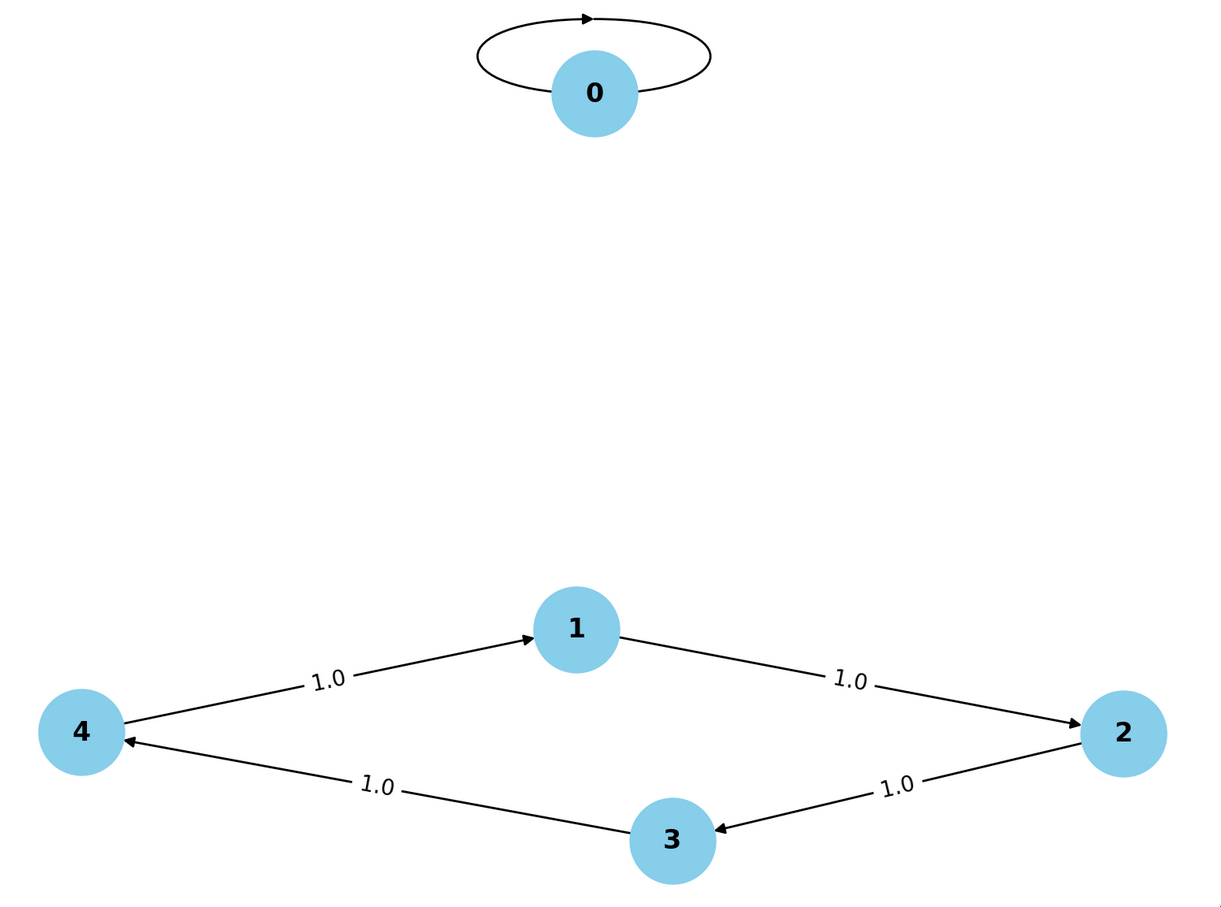
\includegraphics[width=0.8\textwidth]{assets/hw7_problem4.png}
  \caption{solution}
  \label{fig:hw7_problem4}
\end{figure}

\end{proof}
\item Assume that we toss a fair, four-sided die repeatedly. Let $X_n$ be the outcome of the nth toss,
and $S_n = \sum^{n}_{i=1} X_i$. Compute
\[
  \lim_{n \to \infty} P[S_n \text{is divisible by 5}]
.\] 
\begin{proof}
  The 5 states of the markov chain would be the states representing $S_n \mod 5 = \{0,1,2,3,4\}$. The transition matrix $P$ would be 
   \[
     \begin{pmatrix} 0 & \frac{1}{4} & \frac{1}{4} & \frac{1}{4} & \frac{1}{4} \\ \frac{1}{4} & 0 & \frac{1}{4} & \frac{1}{4} & \frac{1}{4} \\ \frac{1}{4} & \frac{1}{4} & 0 & \frac{1}{4} & \frac{1}{4} \\ \frac{1}{4} & \frac{1}{4} & \frac{1}{4} & 0  & \frac{1}{4} \\ \frac{1}{4} & \frac{1}{4} & \frac{1}{4} & \frac{1}{4} & 0 \end{pmatrix}
  .\]
  We know from question 3, that since $P$ is a doubly stochastic matrix, then the stationary distribution vector is just the constant vector. 
   \[
     \vec{v} \cdot P = \vec{v}
  .\] 
  where $\vec{v} = c \cdot \vec{1}$ and  since $\sum_{i=1}^{5} \vec{v}_i = 1$, then $c = \frac{1}{5}$, so
   \[
     \vec{v}^{T} = \begin{pmatrix} \frac{1}{5} \\ \frac{1}{5}\\ \frac{1}{5} \\ \frac{1}{5} \\ \frac{1}{5}  \end{pmatrix}
  .\] 
  The probability that $S_n$ is divisible by $5$ as  $n \to \infty$ is  $S_n \mod 5 = 0$ so  $\lim_{n \to \infty} P[S_n \text{is divisible by } 5 ] = \vec{v}^{T}_{1} = \frac{1}{5}$ representing the probability that this markov chain lands in the state representing a modulus of $0$. 
\end{proof} 

\end{enumerate}

\end{document}
